\section{The Discrete-Time Fourier Transform}
%% subsection
\subsection{Discrete-Time Fourier Transform}
\begin{itemize}
    \item The discrete-time Fourier transform (DTFT) is defined as
    \begin{equation} \label{eqn:dtft}
        X(e^{j\omega}) = \sum_{n=-\infty}^{+\infty} x[n] \ e^{-j\omega n}.
    \end{equation}

    \item Inverse transform
    \begin{align}
        \IDFT 
        &= \frac{1}{2\pi} \int_{-\pi}^{+\pi} \DFT \euler d\omega \\
        &= \lim_{\Delta \omega \to 0} \sum_{k} [X(e^{jk\Delta \omega})\frac{\Delta \omega}{2\pi}]e^{jk\Delta \omega n}
    \end{align}
    Fourier transform is the decomposition of sequences in terms of a linear combination of complex exponentials with incremental amplitudes.

    \item Therefore, the frequency response of a LTI system is the Fourier transform of the impulse response:
    \begin{equation}
        H(e^{j\omega}) = \sum_{n=-\infty}^{+\infty} h[n] \meuler
    \end{equation}
\end{itemize}

%% subsection
\subsection{Properties of DTFT}
\begin{enumerate}

    \item Symmetry properties: 
    \begin{itemize}
        \item If the impulse sequence, $x[n]$ is real, the Fourier transform is a conjugate function:
        \begin{equation}
            \DFT = X^{*}(e^{-j\omega})
        \end{equation}

        \item The magnitude of the Fourier transform, $\lvert X(e^{j\omega}) \rvert$ is an \textit{even} function of $\omega$.

        \item The magnitude of the Fourier transform, $\angle X(e^{j\omega})$ is an \textit{odd} function of $\omega$.
    \end{itemize}
    
    \begin{dv}{}
     Fourier transform:
     \[
      X(e^{j\omega}) =  \sum_{n=-\infty}^{+\infty} x[n] e^{-j\omega n}
     \]
     Replace $\omega$ to $-\omega$:
     \[
      X(e^{-j\omega}) =  \sum_{n=-\infty}^{+\infty} x[n] e^{+j\omega n}
     \]
     Take the complex conjugate of the Fourier transform above: 
     \[
      X^{*}(e^{-j\omega}) =  \sum_{n=-\infty}^{+\infty} \underbrace{x^{*}[n]}_{x[n]} e^{-j\omega n}
     \]
     Since $x[n] \in \mathbb{R}$, the complex conjugate of the Fourier transform is equivalent to Fourier transform:
     \[
      \DFT = X^{*}(e^{-j\omega})
     \]
    \rule{\textwidth}{.1ex}
     Furthermore, express the Fourier transform in terms of a real part and an imaginary part:
     \[
      X(e^{j\omega}) = X_{\mathbb{R}}(e^{j\omega}) + j X_{\mathbb{I}}(e^{j\omega})
     \]
     The complex conjugate of the Fourier transform is thus
     \[
      X^{*}(e^{-j\omega}) = X_{\mathbb{R}}(e^{-j\omega}) - j X_{\mathbb{I}}(e^{-j\omega})
     \]
     Equate the two expressions above, 
     \[
      X_{\mathbb{R}}(e^{j\omega}) = X_{\mathbb{R}}(e^{-j\omega})
     \]
     \[
      X_{\mathbb{I}}(e^{j\omega}) = -X_{\mathbb{I}}(e^{-j\omega})
     \]
     That's saying, the real part of the Fourier transform is an \textit{even} function of $\omega$, and the imaginary part of the Fourier transform is an \textit{odd} function of $\omega$.
    The magnitude of the Fourier transform is an \textit{even} function of $\omega$; the phase of the Fourier transform is an \textit{odd} function of $\omega$.
    \end{dv}
    
    \item Linearity:
    \begin{equation}
        \mathcal{F}\{ax_{1}[n]+bx_{2}[n]\} = a \mathcal{F}\{x_{1}[n]\} + b \mathcal{F}\{x_{2}[n]\}
    \end{equation}

    \item Time and frequency shifting:
    \begin{equation}
        \mathcal{F}\{x[n-n_d]\} = e^{j\omega n_d} \mathcal{F}\{x[n]\}, \quad 
        \mathcal{F}\{e^{j\omega n_d} x[n]\} = X(e^{j(\omega-\omega_n)})
    \end{equation}

    \item Time reversal:
    \begin{equation}
        \mathcal{F}\{x[-n]\} = X^{*}(e^{j\omega})
    \end{equation}

    \item Parseval's theorem:
    \begin{equation}
        \sum_{n=-\infty}^{+\infty} \lvert x[n] \rvert^2 =\frac{1}{2\pi} \int_{-\infty}^{+\infty} \lvert X(e^{j\omega}) \rvert^2 d\omega 
    \end{equation}
    where $\lvert X(e^{j\omega}) \rvert^2$ is the \textit{energy density spectrum} of the sequence, which determines how the energy is distributed in the frequency domain.
    
    \item Convolution
    \begin{equation}
        x[n] * y[n] \leftrightarrow \DFT Y(e^{j\omega})
    \end{equation}
    If 
    \[
        y[n] = \sum_{k=-\infty}^{+\infty} x[k] h[n-k] = x[n] * h[n]
    \]
    Then
    \[
        \mathcal{F} \{y[n]\} = Y(e^{j\omega}) = X(e^{j\omega})H(e^{j\omega})
    \]  
\end{enumerate}

%% subsection
\subsection{Common DTFT Pairs}
\begin{table}[H]
    \centering
    \begin{tabular}{c c}
    \toprule
    $x[n]$    & $X(e^{j\omega})$ \\ 
    \midrule
        $\delta[n]$     &   1  \\[.5em]
        
        1   &   $2\pi \sum_{n=-\infty}^{+\infty} \delta(\omega-2\pi n)$ \\[.5em]
        
        $u[n]$  &   $\frac{e^{j\omega}}{e^{j\omega}-1} \sum_{n=-\infty}^{+\infty} \pi \delta(\omega-2\pi n)$ \\[.5em]
        
        $a^n u[n]$, $\lvert a \rvert <1$    &   $\frac{e^{j\omega}}{e^{j\omega}-a}$ \\[.5em]

        $-a^n u[-n-1]$, $\lvert a \rvert >1$    &   $\frac{e^{j\omega}}{e^{j\omega}-a}$ \\[.5em]

        $a^{\lvert n \rvert}$, $\lvert a \rvert <1$     &   $\frac{1-a^2}{1-2a\cos\omega+a^2}$ \\[.5em]

        $\cos(\omega_0 n)$    &   $\pi \sum_{k=\infty}^{+\infty} [\delta(\omega -\omega_0 - 2\pi k) + \delta(\omega +\omega_0 - 2\pi k)]$ \\[.5em]

        $\sin(\omega_0 n)$    &   $j\pi \sum_{k=\infty}^{+\infty} [\delta(\omega + \omega_0 - 2\pi k) - \delta(\omega - \omega_0 - 2\pi k)]$ \\[.5em]

        $u[n] - u[n-M]$ &   $e^{-j\omega(M-1)/2} (\frac{\sin(M\omega/2)}{\sin(\omega/2)})$\\[.5em]
    \bottomrule
    \end{tabular}
\end{table}

%% subsection
\subsection{From DTFT to DFT}
\begin{itemize}
    \item The discrete-time Fourier transform (DTFT) 
    \[
    X(e^{j\omega}) = \sum_{n=-\infty}^{+\infty} x[n] e^{-i\omega n}
    \]
    is a continuous function of the frequency $\omega$.

    \item If we sample the DTFT (as a continuous function of $\omega$) at $\displaystyle \omega = \frac{2\pi k}{N}$ where $k\in[1, N-1]$, the sampled signal $\Tilde{X_{s}}(j\Omega)$ is:
    \[
    \Tilde{X_{s}}(j\Omega) = X_{s}(j\Omega) \sum_{k=-\infty}^{+\infty} \delta \bigg(k \bigg(\Omega-\frac{2\pi k}{NT} \bigg) \bigg)
    \]
    and the inverse Fourier transform of $\Tilde{X_{s}}(j\Omega)$ is:
    \[
    \Tilde{x}_{s}(t) = NT \sum_{k=-\infty}^{+\infty} x_{s}(t-kNT)
    \]
    As we have observed, $\Tilde{x}_{s}(t)$ is a periodic signal. 

    \item To take one step forward, in terms of the discrete sequence: $\Tilde{x}_{s}(t) \to \Tilde{x}[n]$
    \[
        \Tilde{x}[n] = N \sum_{k=-\infty}^{+\infty} x[t-kN]
    \]
    For $n \in [0, N-1]$, $\Tilde{x}[n]$ is a periodic repetition of $x[n]$. $\Tilde{x}[n]$ is also a periodic signal.
    
    \item This tells us that \textbf{sampling the Fourier transform in the \textit{frequency} domain corresponds to the periodization in the \textit{time} domain}.
    \begin{figure}[H]
        \centering
        \includegraphics{images/DFT_sampling.eps}
        \caption{(a) Finite sequence of $x[n]$; (b) Periodic sequence $\Tilde{x}[n]$ corresponding to the sampling of Fourier transform of $x[n]$}
    \end{figure}
\end{itemize}

\begin{itemize}
    \item Define the discrete Fourier transform (DFT) as the sequence
    \[
        X[k] = X(e^{j\omega})\lvert_{\omega = \frac{2\pi k}{N}} \quad \text{where} \ k=1, 2..., N-1
    \]
    Note: $X[k]$ corresponds to a sampling of the frequency axis.
    
    \item Therefore, the discrete Fourier transform can be expressed as
    \[
        X[k] = \sum_{n=0}^{N-1} x[n] e^{-j 2 \pi kn/N}.
    \]
    
    \item The inverse transform of DFT:
    \[
        x[n] = \frac{1}{N} \sum_{k=0}^{N-1} X[k] e^{j 2 \pi kn/N}.
    \]
\end{itemize}
    
\paragraph{Remarks on DFT and inverse DFT}
\begin{itemize}
    \item[-] The DFT is a sequence that has the same duration as the discrete-time sequence, with a sampled frequency axis.
    \item[-] The DFT is sufficient to reconstruct the original discrete-time series, if the discrete-time series is of finite duration.
\end{itemize}

%% subsection
\subsection{Power Spectral Density}
Power spectral density (power spectrum) is defined as
\[
    PSD[k] = \frac{1}{N}\lvert X[K] \rvert^2 = \frac{1}{N} \bigg \lvert  \sum_{n=0}^{N-1} x[n] e^{-j 2 \pi kn/N}\bigg \rvert^2 
\]
It expressed the power of the signal per unit frequency. 

%% subsection
\subsection{Summary and Example Exam Question}
\begin{figure}[H]
    \centering
    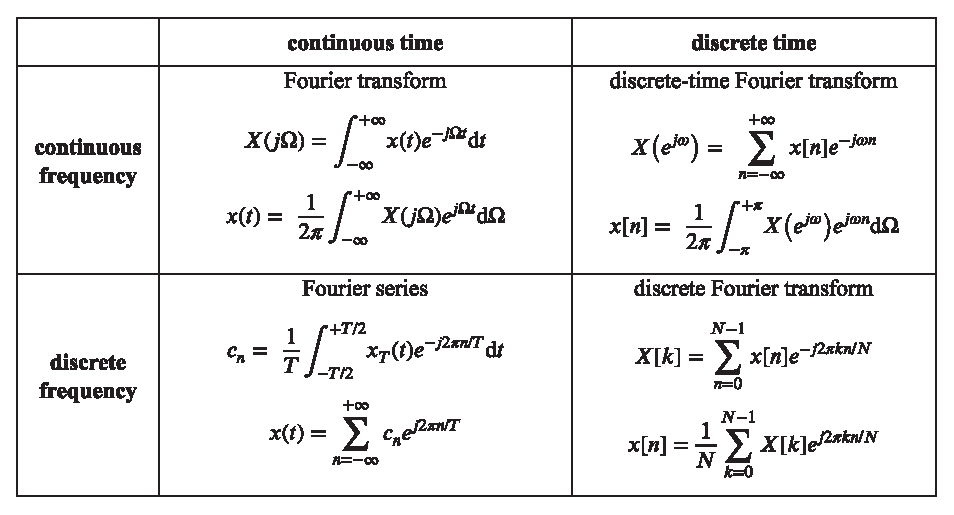
\includegraphics{images/summary_of_FTs.eps}
\end{figure}

\begin{q}{}
    Given the following discrete-time signal:
    \[
        x[n] = 
        \begin{cases}
            1, & n=0 \\
            -3, & n=1 \\
            -1, & n=2 \\
            0, & n=3
        \end{cases}
    \]
    \begin{enumerate}[label=(\alph*)]
        \item Compute the discrete-time Fourier transform $X(e^{j\omega})$.
        \item Compute the discrete Fourier transform $X[k]$ over four points.
    \end{enumerate}
    {\color{blue}
        \paragraph{Answer (a)}
        \begin{align*}
            X(e^{j\omega}) 
            & = \sum_{n=0}^{4} x[n] e^{-j\omega n} \\
            & = 1 - 3e^{-j\omega} - e^{-j2\omega}
        \end{align*}
    }
    {\color{blue}
        \paragraph{Answer (b)}
        \begin{align*}
            X[k] 
            & = X(e^{j\omega})\lvert_{\omega = \frac{2\pi k}{4}} \\
            & = \begin{cases}
                -3, & k = 0\\
                2+3j, & k = 1\\
                3, & k=2 \\
                2-3j, & k=3
            \end{cases}.
        \end{align*}
    }
\end{q}





